\subsubsection{String patching (Win32)}

We can easily find the ``hello, world'' string in the executable file using Hiew:

\begin{figure}[H]
\centering
\myincludegraphics{patterns/01_helloworld/hola_edit1.png}
\caption{Hiew}
\label{}
\end{figure}

And we can try to translate our message into Spanish:

\begin{figure}[H]
\centering
\myincludegraphics{patterns/01_helloworld/hola_edit2.png}
\caption{Hiew}
\label{}
\end{figure}

The Spanish text is one byte shorter than English, so we also added the 0x0A byte at the end (\TT{\textbackslash{}n}) with a zero byte.

It works.

What if we want to insert a longer message?
There are some zero bytes after original English text.
It's hard to say if they can be overwritten: they may be used somewhere in \ac{CRT} code, or maybe not.
Anyway, only overwrite them if you really know what you're doing.

\subsubsection{String patching (Linux x64)}

\myindex{\radare}
Let's try to patch a Linux x64 executable using \radare{}:

\lstinputlisting[caption=\radare{} session]{patterns/01_helloworld/radare.lst}

Here's what's going on: I searched for the \q{hello} string using the \TT{/} command,
then I set the \emph{cursor} (\emph{seek}, in \radare{} terms) to that address.
Then I want to be sure that this is really that place: \TT{px} dumps bytes there.
\TT{oo+} switches \radare{} to \emph{read-write} mode.
\TT{w} writes an ASCII string at the current \emph{seek}.
Note the \TT{\textbackslash{}00} at the end---this is a zero byte.
\TT{q} quits.

\subsubsection{This is a real story of software cracking}
\myindex{\SoftwareCracking}

An image processing software, when not registered, added watermarks,
like ``This image was processed by evaluation version of [software name]'', across a picture.
We tried at random: we found that string in the executable file and put spaces instead of it.
Watermarks disappeared.
Technically speaking, they continued to appear.
\myindex{Qt}
With the help of Qt functions, the watermark was still added to the resulting image.
But adding spaces didn't alter the image itself...

\subsubsection{Software \emph{localization} of MS-DOS era}
\myindex{MS-DOS}

This method was a common way to translate MS-DOS software to Russian language back to 1980's and 1990's.
This technique is available even for those who are not aware of machine code and executable file formats.
The new string shouldn't be bigger than the old one, because there's a risk of overwriting another value or code
there.
Russian words and sentences are usually slightly longer than its English counterparts, so that is why \emph{localized}
software has a lot of weird acronyms and hardly readable abbreviations.

\begin{figure}[H]
\centering
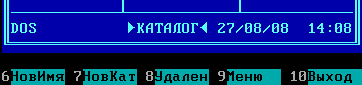
\includegraphics[width=0.5\textwidth]{patterns/01_helloworld/Norton_Commander_v5_51.png}
\caption{\emph{Localized} Norton Commander 5.51}
\end{figure}
% note to translators: if you know such examples of MS-DOS programs 'localized' to your native language,
% please tell me, maybe I will add more screenshots.

Perhaps this also happened to other languages during that era, in other countries.

\myindex{Borland Delphi}
As for Delphi strings, the string's size must also be corrected, if needed.
